\chapter{Introduction}\label{c:intro}

Simple arithmetic skills are difficult to master. Although we understand
arithmetic well intellectually, we falter in its execution. As Marr put it:
``I have no doubt that when we do mental arithmetic we are doing something
well, but it is not arithmetic'' \citeyear[p.~348]{marrviso}. Children have
acquired a
host of impressive skills by the time they are taught formal arithmetic:
they have learned a language and can use vision for autonomous navigation
in a hostile environment. In contrast, the ``simple'' tasks of arithmetic
require at least a further five or six years of schooling. Once the skills
are learned there are many opportunities for error. Adults, for example,
make plenty of mistakes recalling multiplication facts---especially on the
``tricky'' problems, such as \x84 or \x98. Arithmetic, it seems, is not an
easy skill to come by.

So what is the ``something'' that we do well when we solve arithmetic
problems? The view taken here is that the things we do well are those tasks
suited to a certain kind of computation---namely connectionism. Difficult
tasks, such as arithmetic, need to be turned into pattern matching
problems.  That is, ``we succeed in solving logical problems not so much
through the use of logic, but by making the problems we wish to solve
conform to problems we are good at solving'' \cite[p.~44]{pdp:14}. Exactly
how this is done for arithmetic is the topic of this thesis. Two elementary
arithmetic skills are considered: adult memory for multiplication facts and
children's errors in long (multicolumn) multiplication.


\section{Part I---Mental arithmetic}

The first part of the thesis considers recall of multiplication
facts, such as \xeq{3}{6}{18}.  Intuitively it seems that recalling the
answer to such a problem is neither difficult nor drawn-out. However, the
model presented here suggests a brief struggle between products in memory
before the (often correct) answer ``pops up.'' As problems get more
difficult, which usually means larger, the struggle takes a little
longer---around one second in some cases. Certain problems are easier than
others, notably the tie problems (\x22, \x33, and so on), and the 5s
problems (5 times anything).  When mistakes are made they tend to be
related to the presented problem.  For example, a common mistake is
\xeq{6}{7}{48}, and 48 is the answer to \x{6}{8}.  That is, errors are
often the correct answer for a problem which shares an operand with the
presented problem.

This phenomenon and previous models are looked at in detail in
chapter~\ref{c:xlit}. The review draws on normal and brain-damaged studies
of the reaction times and errors of adults recalling multiplication facts.

Chapter~\ref{c:xnet} describes the connectionist model built to capture
the reaction times and errors of adults.  The basic idea is a simple one:
memory for multiplication facts consists of a set of associations between
operands and products; recall is the process of spreading activation,
resulting in a product's activation
exceeding a threshold.  The activation spreads at
different rates for different problems, giving different reaction times.
Occasionally, when under some kind of time pressure, a false product
exceeds the threshold.  Most of these errors are operand errors, and the
reasons for this are explored.

By varying the assumptions of the simulations,
certain factors were found
to be important in determining the phenomena.   There is
some evidence that
smaller problems are experienced more often than larger problems, and this
skew in frequency has a strong effect on the model.  Also, the input
encoding to the network (representing the operands of a problem) can effect
the distribution of errors and reaction times. In particular,
the degree of ``coarseness'' or ``sharpness'' of the encoding is explored.

Other phenomena are also investigated.  For example, it seems that zero
problems (zero times anything) are solved by the rule \xeq{0}{N}{0}.  There
is plenty of evidence for this, including: zero problems are solved very
quickly; errors are of the form \xeq{0}{N}{N}; brain-damaged patients can
re-learn zero problems from exposure to just 2 examples, but not
non-zero problems.  There is certainly something special about zero, and it
is not clear how this fits into the
associative framework.


\section{Part II---Multicolumn multiplication}

The second half of the thesis examines children's errors on
multicolumn multiplication problems.  Behaviour on these problems seems to
be rule governed. Children pick up a collection of
``bugs''---systematic perturbations to the correct rules of arithmetic---
and apply the rules producing all sorts of errors. For example:

\begin{arithprob}{p{1em}p{1em}p{1em}p{1em}}
$\ _{\ }$&$5_{\ }$&$2_{\ }$&$4_{\ }$\\
$\times$$\ _{\ }$&$7_{\ }$&$3_{\ }$&$1_{\ }$\\
\cline{1-4}$3_{\ }$&$5_{\ }$&$6_{\ }$&$4_{\ }$\\
\end{arithprob}
\hspace{2cm}
\begin{arithprob}{p{1em}p{1em}p{1em}}
$\ _{\ }$&$7_{\ }$&$6_{\ }$\\
$\times$$\ _{\ }$&$\ _{\ }$&$4_{\ }$\\
\cline{1-3}$1_{\ }$&$4_{2}$&$4_{\ }$\\
\end{arithprob}\skipafterprob

In the first example, the child multiplies using the pattern for addition:
\xeq{1}{4}{4}, \xeq{3}{2}{6}, \xeq{7}{5}{35}.  The second example shows a
child getting the first multiplication, \xeq{4}{6}{24}, correct. Then,
when there is no second multiplier, the child uses the carry in the next
multiplication: \xeq{2}{7}{14}.

These errors have previously been modelled with production systems.
Chapters~\ref{c:bugs} reviews the literature on buggy behaviour and models
of buggy behaviour, and outlines relevant work from connectionism.
Particular attention is paid to VanLehn's
\citeyear{mindbugs} ``Sierra'' model, as this seems to be the best
available model of procedural misconceptions \cite<see also>{pirobook}.
Briefly, the prevailing notion is that children reach ``impasses'' when
solving problems---situations in which no rules directly apply.
These impasses need
to be ``repaired'' by general purpose heuristics.  Sierra has these
heuristics and a learning mechanism. Incomplete arithmetic rules are
learned, which means that Sierra reaches impasses.  Different errors are
observed depending on what kind of repair is carried out.

Sierra is a successful model, and the mistakes children make they do seem to
derive from following faulty rules. How could a connectionist
build a model of this behaviour? As \citeA[p.~167]{bodecomp} notes:
\begin{ssquote}
It is not clear that processes of relaxation using multiple
constraints, powerful though they may be for pattern matching, are
well suited to modelling conscious planning or cryptarithmetic---or
even mere arithmetic, for that matter.
\end{ssquote}

Chapter~\ref{c:fsm} explains the approach taken in giving a
connectionist interpretation of multicolumn arithmetic.

A set of operations was devised to allow a network to move around, read
from and write on a problem.  A ``curriculum'' of problems was selected,
starting with easy addition tasks and moving up to three column
multiplication.  Each problem was encoded as a sequence of operations and a
recurrent network was trained to activate the correct operation at the
correct moment when solving a problem.  Buggy behaviour was exhibited when
the network was tested on unseen problems.  Analysis shows that the
representations learned by the model have a procedural structure, allowing
bugs to be composed of correct skills plus chunks of skills which are
correct in other situations.  It is suggested that the gradual learning of
these representations is an interesting alternative to snap-shot rule
acquisition accounts.

Connectionist models do not reach impasses as such.  That is, there is
never a moment when the system ``gets stuck'' and needs to repair the
current state.  Hence it is necessary to address the role of impasses in
learning this task. Are impasses important learning events, or just a
by-product of the problem solving mechanism?

It was never going to be possible to build a model which could compete with
the empirical power of VanLehn's system: Sierra is the product of
over ten years research.  Rather, the work described in this half of the
thesis is best thought of as a ``demonstrator'' of how one might model
arithmetic from a connectionist perspective.

\section{Structure of arithmetic skills}

The splitting of arithmetic skills into two models---fact recall and
procedural skills---is supported by studies of brain-damaged subjects
\cite{mcclcogn,mcclfact}. Figure~\ref{f:numstruct} shows the structure of
the number-processing system.  This structure was devised by noting that
particular components of the system can be selectively damaged. For
example, one subject (RR) was asked to read Arabic numbers aloud. For
37~000 he said ``Fifty-five thousand'', for 2 he said ``one''
\cite[pp.~187--188]{mcclcogn}. Yet RR could determine which of two
presented numbers was larger, and had no trouble selecting a pile of tokens
that corresponded to a presented Arabic number.  It seems that RR had no
difficulty in comprehending and representing number, but was impaired in
production alone.

This, and other experiments, led \citeA{mcclcogn} to propose the structure
shown in figure~\ref{f:numstruct}.  The model of arithmetic memory deals
with the ``arithmetic facts'' and ``abstract representation'' parts of the
figure.  The multicolumn model is concerned with the ``calculation
procedures'' part of the structure.

\begin{fancyfigure}
\centerline{\psfig{file=structure.ps,height=7.5cm}}
\caption{The structure of the cognitive number processing system
\protect\cite<after>[figure~1]{mcclfact}.}
\label{f:numstruct}
\end{fancyfigure}

\section{Aims}

There are two major aims. First, to build an explicitly specified model of
memory for multiplication facts.  Previous models have been poorly
specified---either not implemented at all, or making assumptions such as
the probability of an error being proportional to answer node activation.
These details need to be fleshed out in order to understand the importance
of various assumptions, or changes to assumptions.  Hence, the first
contribution is an explicit model that can be tested and criticised.
Variations on the model aim to understand the causes of the phenomenon.
The causes include the frequency of problems, the creation of false
associations and the nature of the facts themselves.

The second aim is to demonstrate
an alternative to production system models of
multicolumn arithmetic, and to show that such an approach is useful.  This
constitutes the first connectionist model of this phenomena. Errors are
characterized as perturbations to processing trajectories, rather than faulty
rules or repairs to impasses.  This view conceptualizes learning as the
formation and differentiation of states in something similar to a finite
state machine.
In addition, the analysis of the
system is a useful analysis of a sequential
network learning a large structured problem.
